\chapter{Introduction}
\section{Motivation}
In the first half of the twentieth century, Walter Shewart pioneered the use of statistical control charts for detecting real-time changes in variation.  Shewart was interested in reducing the unexpected causes of variation in the manufacturing processes that produced faulty manufacturing equipment \cite{shewhart1931economic}. Shewart's method involved charting the process measurements over time and detecting when a statistical process was no longer exhibiting an expected level of variation. Once this detection occurred, the process was stopped and was not restarted until the cause of the variation was fixed.
Shewart's control charts were one of the first formal methods to solve the problem of detecting changes in a distribution of a sequence of random variables. This problem is now known more generally as the \textit{change point detection problem}. Many industries make use of change point techniques for real-time decision support systems. The following are a few motivating examples.

\subsection{Health Care}
Health care is an important area for quickly detecting signal changes. Some recent studies include applications to heart rate monitoring \cite{yang2006adaptive} \cite{staudacher2005new}, epilepsy signal segmentation \cite{malladi2013online}, and multi-modal MRI lesion detection \cite{bosc2003automatic} to name a few. Quickly detecting changes to a patient's health is absolutely necessary for any system to be of practical use. However, this quick detection must be balanced with high accuracy as false positives or missed detections could have life-threatening consequences. Therefore, balancing missed change points with  falsely identified change points is a central theme to online change point detection.

%\subsection{Computer Network Surveillance}
%Networks/monitoring systems for intrusions and/or changes in climate or natural disasters.

\subsection{Financial Applications}
The application of accurate and timely change point detection is popular in the finance sector where shifts in asset prices can suddenly happen. Change point detection is particularly hard in financial applications because of the non-stationary data typically observed in asset price time series. A common goal is detecting key, historical moments in the market such as stock market crashes \cite{banerjee2020change}  or the sub-prime mortgage crisis \cite{zhu2015change}. Note, in the financial literature, change points  are also referred to as structural breaks, but for this thesis we will use the broader term change points.

One example of an online, quick detection technique is proposed in  \cite{pepelyshev2017real}, where a modified Shiryaev - Roberts procedure is used to detect a change point in a single stock's daily returns. See Figure \ref{fig:apple} for the kind of of change points the authors try to detect. They compare their non-parametric method with other classic control chart methods using speed of detection and false alarm rate as measures of performance.
\begin{center} 
\captionof{figure}[Daily Price and Return for AAPL]{Daily stock prices (\textbf{top}) and daily returns (\textbf{bottom}) for Apple Inc. (NYSE: AAPL) for the period from January 1, 2006 through February 28, 2020.} 
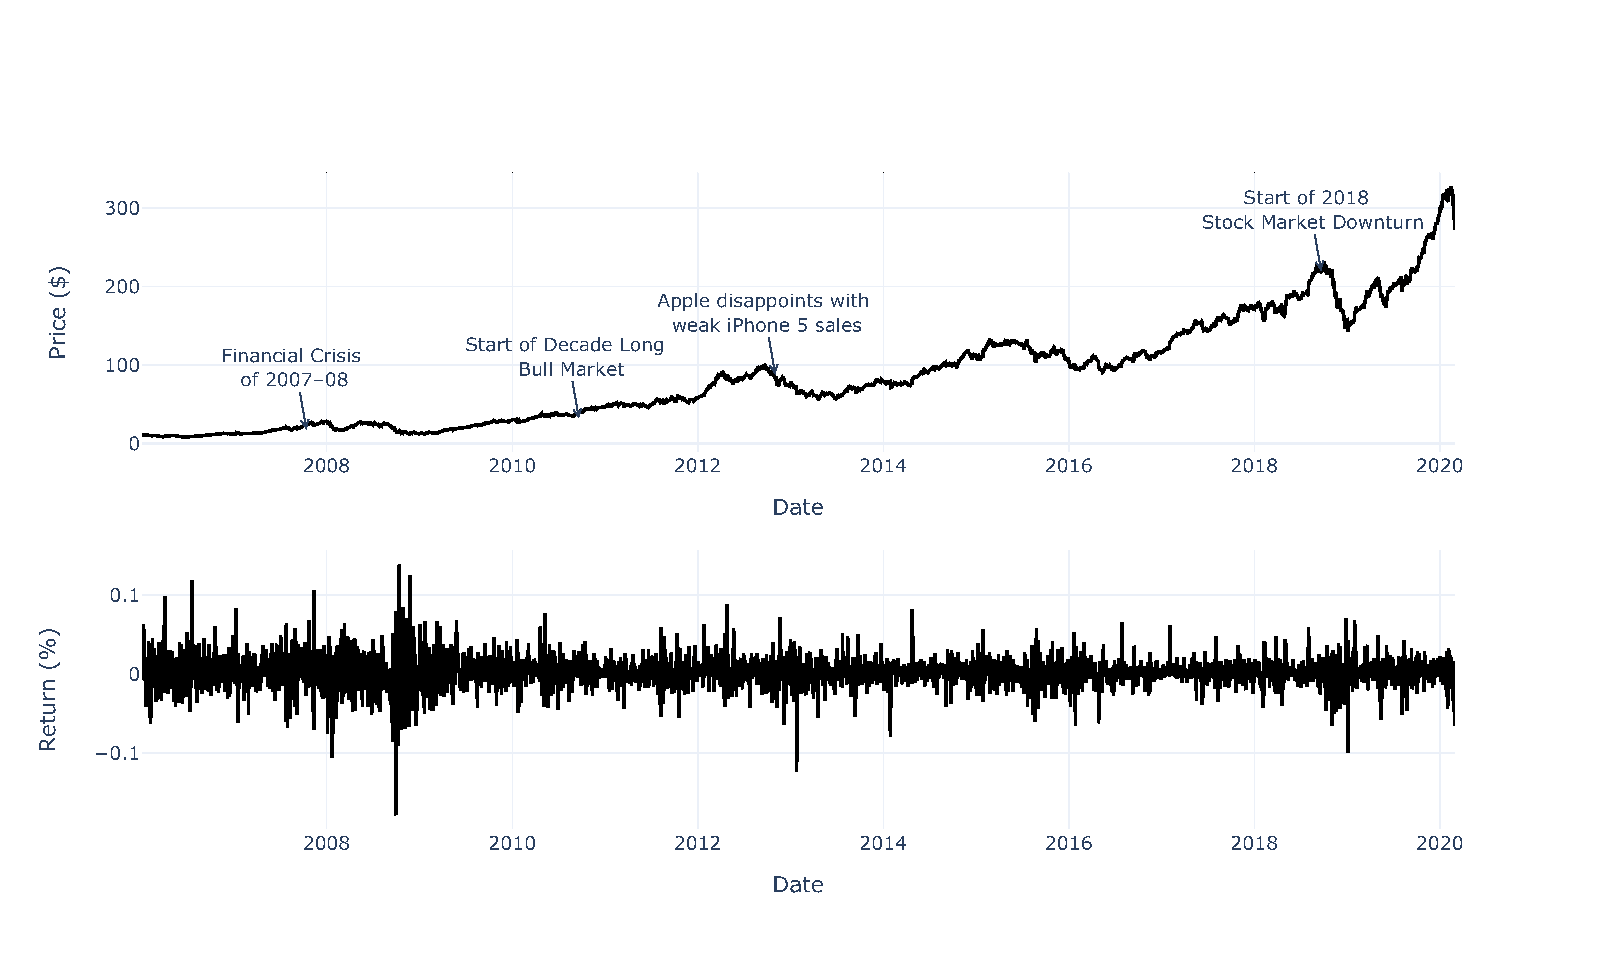
\includegraphics[trim=0cm 1cm 0cm 1cm, clip, width=\textwidth]{apple_returns} 
\label{fig:apple} 
%\medskip
%\tiny
%(top) Daily stock prices (at closing) and (bottom) Daily returns on the stock (evaluated at closing) of Apple Inc. 
\end{center}

Detecting changes in variance is explored in  \cite{lavielle2007adaptive}. The authors propose an offline change point algorithm that minimizes a global cost function by using an adaptive regularization function. The algorithm is applied to the absolute returns of the FTSE 100 stock index and the US dollar-Japanese Yen foreign intra-day exchange rate to detect changes in asset price volatility. The change points  identified in the FTSE 100 coincided with key market events such as the stock market crash that occurred on October 14$^{th}$, 1987 and breaking the 5000 price barrier in August 1997.

% This guy did some modified CUSUM type tests do equity and FX returns http://www.long-memory.com/volatility/AndreouGhysels2002.pdf
% very statistical approach using arch models and other parametric assumptions, they use some tick data, so that's cool

For more applications to options markets and arbitrage opportunities, see section 1.3.6 of \cite{tartakovsky2014sequential}.


\section{Characteristics of the change point problem}
A number of surveys of the literature already exist \cite{aminikhanghahi2017survey} \cite{niu2016multiple}, therefore we will not cover all existing methods but rather touch upon several, important factors to consider when approaching a change point detection problem. Across the literature, these factors determine what methods are available to practitioners. %Furthermore, Bayesian methods that relate to change point detection but will not be covered in this thesis.

The first factor is selecting between \textit{parametric} and \textit{non-parametric} techniques. Deciding between these two broad techniques is dependent on the prior knowledge one wants to encode into the problem. For example, if it is known that data is generated by a distribution from an exponential family of distributions, then the problem can be subsetted from the space of all possible distributions to a smaller space of distributions. For example, Shewart control charts and CUSUM change point techniques are both parametric techniques based on the Gaussian-family of distributions \cite{page1954continuous} \cite{chen2011parametric}. In other settings, it is not possible to leverage information about the data and non-parametric techniques must be used instead \cite{brodsky2013nonparametric}.

% . On the other hand, if the data is being generated by processes that have no fundamental or well-understood process then modelling particular probability distributions becomes intractable or risky. Therefore, models that do not model particular probability distributions must be used. For reference, see monograph by Brodsky and Darkhovsky \cite{brodsky2013nonparametric}. % Usually this added flexibility is a trade-off with performance and/or speed with parametric models.

The second factor is deciding whether change points should be detected \textit{offline} or \textit{online}. Some algorithms are offline---also referred to  as batch algorithms or retrospective or \textit{posteriori} change point detection---and they are applied in an ex-post fashion after the dataset has been completely acquired \cite{truong2020selective}. If change points must be detected as soon as possible, then waiting for the entire dataset to be acquired is not feasible and methods that operate on data streams must be used. Methods that fall into the category are referred to as online change point detection methods. The aforementioned Shewart control chart and CUSUM algorithm are both designed for data that is streamed in real-time. In the statistical literature, online methods of change point detection are also referred to sequential change point detection  \cite{tartakovsky2014sequential}. For this thesis, the terms will be used interchangeably.% For an exhaustive review of sequential change point analysis, see the book by Tartakovsky, Nikiforov, and Basseville  \cite{tartakovsky2014sequential}. %It is possible to convert an online algorithm to an offline algorithm by simply 

%The third consideration that is a consequence of detecting change points in an online setting is the presence of outliers. This a particularly important concern for online methods that are looking for changes in the underlying distribution of points, not a single anomalous data point

The third factor is determining if there are multiple change points or only one change point to detect. This is an important  factor for offline change point detection where the decision to detect one or more change points is often chosen at the outset \cite{jandhyala2013inference}.  Detecting multiple change points could also be relevant for the online case if a situation arises where the window of time series under consideration may contain more than one change point. However, most online change point methods are designed to detect a single change point at a time.

Finally, the last factor to address is determining what statistical changes a detection algorithm should detect. Many methods focus solely on detecting changes in the mean of a distribution \cite{lee2010change} or changes in variance \cite{hawkins2005change} \cite{inclan1994use}. Methods like kernel change point detection do not focus on detecting a specific statistical parameter, but rather detecting that a change occurred in some moment of the distribution \cite{arlot2019kernel}. This is especially useful in situations where very little is known about the data.

This thesis will concern itself with online change point detection, where data is received in a streaming nature. We assume no prior distributional characteristics on the data and operate in a completely non-parametric setting. 


\section{Our Contributions}
The contributions of this work are several fold. First, to our knowledge, no paper has applied change point techniques to a financial instrument's market liquidity by evaluation of regime changes in the limit order book (LOB). Second, given the strong emphasis of theoretical results in the change point detection community, we test several, recent online kernel change point algorithms on several synthetic datasets. Expected detection delay, false alarm rate and missed detections are compared across the various methods. The focus of recent algorithms is on kernel methods such as KCUSUM, NEWMA and Scan-B that will be discussed in detail in chapter \ref{chapter3}. Thirdly, we demonstrate an online median algorithm that can be used for tuning the Gaussian kernel bandwidth when it's used for kernel change point detection. Several use cases where performance is superior with this online median bandwidth selection is shown as well. 

\section{Chapter Overview}
Below is a short description of each chapter and its contents. %Ideally, each chapter should be read chronologically, but effort has been made so that each chapter is as self-contained as possible.

Chapter 2 provides a background on hypothesis testing and its relation to the change point detection problem. The online change point problem is formulated along with measures for evaluating performance. The chapter closes out by reviewing classic methods for detecting change points on streaming data.

Chapter 3 examines kernel change point detection as it is a focus of this thesis. A short background on the maximum mean discrepancy and its use in two-sample hypothesis tests is covered first. This is followed by a review of the most competitive online, kernel change point detection methods. It concludes with a novel way to estimate the kernel bandwidth for online methods.

Chapter 4 constructs several synthetic datasets for experimentation. Results are compared across several kernel change point methods and across several performance metrics. Particular use cases for the novel technique presented in the previous chapter are presented as well.

Chapter 5 applies a kernel change point detection algorithm to market liquidity in financial markets. A model of the limit order book is presented and the construction of the financial dataset is explained.

Chapter 6 concludes the thesis by summarizing all the results and discussing future avenues for research.
